%% Creator: Inkscape inkscape 0.92.3, www.inkscape.org
%% PDF/EPS/PS + LaTeX output extension by Johan Engelen, 2010
%% Accompanies image file 'Concept_mininal.pdf' (pdf, eps, ps)
%%
%% To include the image in your LaTeX document, write
%%   \input{<filename>.pdf_tex}
%%  instead of
%%   \includegraphics{<filename>.pdf}
%% To scale the image, write
%%   \def\svgwidth{<desired width>}
%%   \input{<filename>.pdf_tex}
%%  instead of
%%   \includegraphics[width=<desired width>]{<filename>.pdf}
%%
%% Images with a different path to the parent latex file can
%% be accessed with the `import' package (which may need to be
%% installed) using
%%   \usepackage{import}
%% in the preamble, and then including the image with
%%   \import{<path to file>}{<filename>.pdf_tex}
%% Alternatively, one can specify
%%   \graphicspath{{<path to file>/}}
%% 
%% For more information, please see info/svg-inkscape on CTAN:
%%   http://tug.ctan.org/tex-archive/info/svg-inkscape
%%
\begingroup%
  \makeatletter%
  \providecommand\color[2][]{%
    \errmessage{(Inkscape) Color is used for the text in Inkscape, but the package 'color.sty' is not loaded}%
    \renewcommand\color[2][]{}%
  }%
  \providecommand\transparent[1]{%
    \errmessage{(Inkscape) Transparency is used (non-zero) for the text in Inkscape, but the package 'transparent.sty' is not loaded}%
    \renewcommand\transparent[1]{}%
  }%
  \providecommand\rotatebox[2]{#2}%
  \newcommand*\fsize{\dimexpr\f@size pt\relax}%
  \newcommand*\lineheight[1]{\fontsize{\fsize}{#1\fsize}\selectfont}%
  \ifx\svgwidth\undefined%
    \setlength{\unitlength}{278.47127013bp}%
    \ifx\svgscale\undefined%
      \relax%
    \else%
      \setlength{\unitlength}{\unitlength * \real{\svgscale}}%
    \fi%
  \else%
    \setlength{\unitlength}{\svgwidth}%
  \fi%
  \global\let\svgwidth\undefined%
  \global\let\svgscale\undefined%
  \makeatother%
  \begin{picture}(1.0,1.75) %1.89882926)%
    \lineheight{1}%
    \setlength\tabcolsep{0pt}%
    \put(0,0){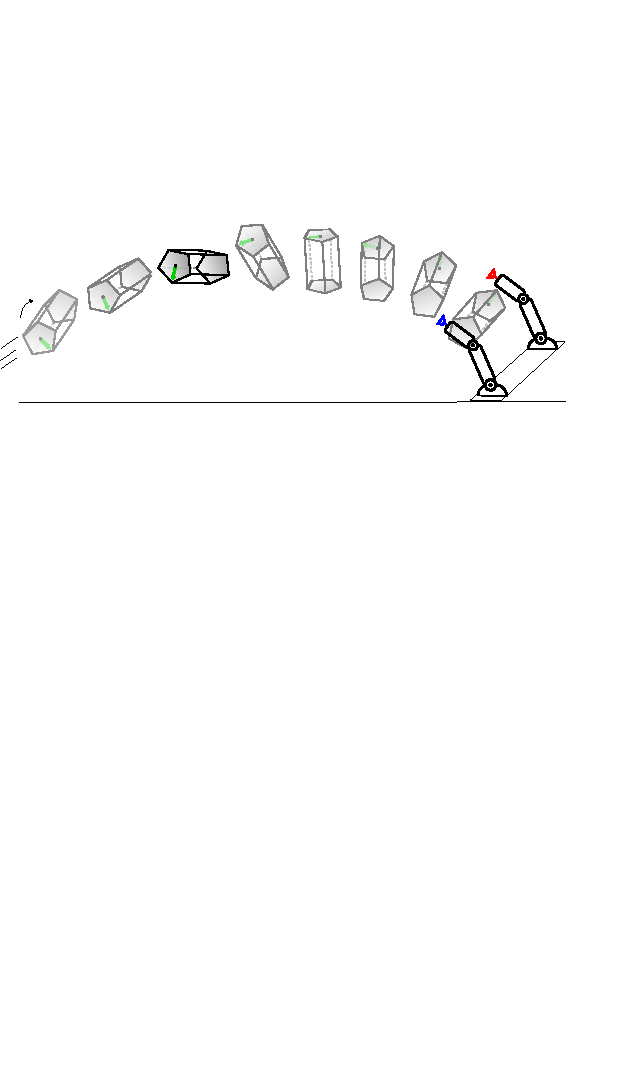
\includegraphics[width=\unitlength,page=1]{images/Concept_mininal1.pdf}}%
    \put(0.40,1.7){\color[rgb]{0,0,0}\makebox(0,0)[lt]{\lineheight{0.60000002}\smash{\begin{tabular}[t]{l}\textbf{Estimation}\end{tabular}}}}%
    \put(0.30,1.5){\color[rgb]{0,0,0}\makebox(0,0)[lt]{\lineheight{0.60000002}\smash{\begin{tabular}[t]{c}$\dot{\bm{x}}_t$\end{tabular}}}}%
    
    \put(0,0){\includegraphics[width=\unitlength,page=2]{images/Concept_mininal1.pdf}}%
    \put(0.40,1.41){\color[rgb]{0,0,0}\makebox(0,0)[lt]{\lineheight{0.60000002}\smash{\begin{tabular}[t]{l}\textbf{Prediction}\end{tabular}}}}%
    % \put(0.35,1.175){\color[rgb]{0,0,0}\makebox(0,0)[lt]{\lineheight{0.70000002}\smash{\begin{tabular}[t]{c}$\bm{x}_i, \dot{\bm{x}}_i$ \\\\ $\forall i=\{t+1,...,t+l\}$\end{tabular}}}}%
    
    \put(0,0){\includegraphics[width=\unitlength,page=3]{images/Concept_mininal1.pdf}}%
    \put(0.37,1.05){\color[rgb]{0,0,0}\makebox(0,0)[lt]{\lineheight{0.60000002}\smash{\begin{tabular}[t]{l}\textbf{Contact Selection}\end{tabular}}}}%
    \put(0.55,0.8){\color[rgb]{0,0,0}\makebox(0,0)[lt]{\lineheight{0.90000002}\smash{\begin{tabular}[t]{c}$\mathbf{p}_j$ \end{tabular}}}}%
    % \put(0.475,0.75){\color[rgb]{0,0,0}\makebox(0,0)[lt]{\lineheight{0.90000002}\smash{\begin{tabular}[t]{c}$j \approx t+\tau$\end{tabular}}}}%
    % \put(0.8, 0.94){\color[rgb]{0,0,0}\makebox(0,0)[lt]{\lineheight{0.60000002}\smash{\begin{tabular}[t]{l}\tiny{workspace}\end{tabular}}}}%
    
    \put(0,0){\includegraphics[width=\unitlength,page=4]{images/Concept_mininal1.pdf}}%
    \put(0.33181408,0.7){\color[rgb]{0,0,0}\makebox(0,0)[lt]{\lineheight{0.60000002}\smash{\begin{tabular}[t]{l}\textbf{Impact-aware planning}\end{tabular}}}}%
    \put(0.3, 0.43){\color[rgb]{0,0,0}\makebox(0,0)[lt]{\lineheight{0.60000002}\smash{\begin{tabular}[t]{c}\tiny{make contact} \\ \tiny{low stiffness}\end{tabular}}}}%
    \put(0.9, 0.685){\color[rgb]{0,0,0}\makebox(0,0)[lt]{\lineheight{0.60000002}\smash{\begin{tabular}[t]{c}\tiny{motion plan} \end{tabular}}}}%
    \put(0.77, 0.65){\color[rgb]{0,0,0}\makebox(0,0)[lt]{\lineheight{0.60000002}\smash{\begin{tabular}[t]{c}$\bm{q}_i, \bm{K}_i$ \end{tabular}}}}%
    % \put(0.67, 0.62){\color[rgb]{0,0,0}\makebox(0,0)[lt]{\lineheight{0.60000002}\smash{\begin{tabular}[t]{l}\tiny{$\forall i=\{j,...,j+\nu\}$}  \end{tabular}}}}%
    
    %   

    \put(0,0){\includegraphics[width=\unitlength,page=5]{images/Concept_mininal1.pdf}}%
    \put(0.36,0.322){\color[rgb]{0,0,0}\makebox(0,0)[lt]{\lineheight{0.60000002}\smash{\begin{tabular}[t]{l}\textbf{Compliant catching}\end{tabular}}}}%
    \put(0.3, 0.06){\color[rgb]{0,0,0}\makebox(0,0)[lt]{\lineheight{0.60000002}\smash{\begin{tabular}[t]{c}\tiny{stable contact} \\ \tiny{high stiffness}\end{tabular}}}}%
    \put(0.75, 0.25){\color[rgb]{0,0,0}\makebox(0,0)[lt]{\lineheight{0.60000002}\smash{\begin{tabular}[t]{c}\tiny{tracking plan}\end{tabular}}}}%
    \put(0,0){\includegraphics[width=\unitlength,page=6]{images/Concept_mininal1.pdf}}%
  \end{picture}%
\endgroup%
